%%%%%%%%%%%%%%%%%%%%%%%%%%%%%%%%%%%%%%%%%%%%%%%%%%%%%%%%%%%%%%%%%%%%%%%%%%%%%%%
\chapter{Flusso su corpi}\label{chp:FlowBodieas}
%%%%%%%%%%%%%%%%%%%%%%%%%%%%%%%%%%%%%%%%%%%%%%%%%%%%%%%%%%%%%%%%%%%%%%%%%%%%%%%

Un fluido in movimento apporta forze di pressione normali ad un corpo immerso e forse tangenziali alla superficie.
Per un flusso bidimensionale, la risultante della pressione e forze di taglio possono essere considerate in due componenti:
\begin{itemize}
\item \eng{Drag force} in direzione del flusso;
\item \eng{Lift force} in direzione normale al flusso.
\end{itemize}
Nel caso di un flusso tridimensionale c'è una componente mista normale al piano \eng{drag-lift}.
Allora, le forze possono generare anche dei momenti come:
\begin{itemize}
\item momento di rollio,
\item momento di beccheggio,
\item momento di bardata.
\end{itemize}

\begin{equation}
\begin{split}
F_D &= \int_A{\left(-p\cos\theta + \tau_W\sin\theta\right)\,dA}\\
F_L &= -\int_A{\left(p\sin\theta + \tau_W\cos\theta\right)\,dA}
\end{split}
\end{equation}

\begin{figure}
\centering
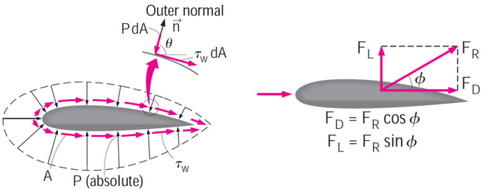
\includegraphics[width = \textwidth]{gfx/DragLift}
\caption{Scomposizione delle forze su un profilo alare in \eng{drag} e \eng{lift}}
\label{fig:DragLift}
\end{figure}

Sia la frizione superficiale sia la pressione, in generale, contribuiscono a $F_D$ e $F_L$. In caso di una lastra piana fina allineata parallela alla direzione del flusso, $F_D$ dipende solamente dalle forze di taglio.
Quando la lastra è normale alla direzione del flusso $F_D$ dipende solo dalla pressione.

\section{Coefficienti di drag e lift}
i coefficienti di \eng{drag} e \eng{lift} sono definiti come:
\begin{equation}
C_D = \frac{F_D}{\rho \frac{V^2}{2}A} \qquad C_L = \frac{F_L}{\rho \frac{V^2}{2}A}
\end{equation}
I due coefficienti rappresentano il comportamento di \eng{drag} e \eng{lift} del corpo.
In generale dipendo dalle caratteristiche geometriche del corpo. Dipendono anche dal numero di Reynolds e dalla rugosità della superficie.
I coefficienti locali, variano lungo la superficie in finzione dei cambiamenti della velocità dello strato limite nella direzione di flusso.
Si può definire i coefficienti medi del corpo nel momento in cui sono disponibili i coefficienti locali lungo tutta la lunghezza della superficie. 
Possono dipendere anche dal numero di Mach, a patto che sia rilevante per la geometria: $Ma \geq 0.3$.

\subsection{Composizione drag}
La forza di \eng{drag} è composizione di diversi fenomeni:
\begin{description}
\item[Frizione] dovuta prevalentemente dagli sforzi di taglio sulla parete $\tau_W$. Causata da effetti d'attrito.
\item[Pressione] dovuta al contributo della pressione sul profilo. Definita anche dalla forte dipendenza dalla geometria del corpo.
\end{description}
Si può definire:
\begin{equation}
F_D = F_{D, \textup{Friction}} + F_{D, \textup{Pressure}} \qquad C_D = C_{D, \textup{Friction}} + C_{D, \textup{Pressure}}
\end{equation}
%*****************************************
\chapter{Aerodinamica di un profilo alare}\label{ch:Airfoil}
%*****************************************
